%%% LaTeX Template: Article/Thesis/etc. with colored headings and special fonts
%%%
%%% Source: http://www.howtotex.com/
%%% Feel free to distribute this template, but please keep to referal to http://www.howtotex.com/ here.
%%% February 2011
%%%
%%% Modified May 2018 by CDM

%%%  Preamble
\documentclass[11pt,letterpaper]{article}
\usepackage[margin=1.0in]{geometry}
\usepackage[T1]{fontenc}
\usepackage[bitstream-charter]{mathdesign}
\usepackage[latin1]{inputenc}					
\usepackage{amsmath}						
\usepackage{xcolor}
\usepackage{cite}
\usepackage{hyphenat}
\usepackage{graphicx}
\usepackage{float}
\usepackage{subfigure}
\usepackage{sectsty}
\usepackage[compact]{titlesec} 
\usepackage[tablegrid]{vhistory}
\allsectionsfont{\color{accentcolor}\scshape\selectfont}

%%% Definitions
\definecolor{accentcolor}{rgb}{0.0,0.0,0.5} 
\newcommand{\teamname}{Team IDP}
\newcommand{\productname}{MavDegreePlanner}
\newcommand{\coursename}{CSE 4316: Senior Design I}
\newcommand{\semester}{Fall 2021}
\newcommand{\docname}{System Requirements Specification}
\newcommand{\department}{Department of Computer Science \& Engineering}
\newcommand{\university}{The University of Texas at Arlington}
\newcommand{\authors}{Daniel Newville \\ Le Uyen Nguyen \\ Ijaz Mohamed Umar \\ Safi Ullah}

%%% Headers and footers
\usepackage{fancyhdr}
	\pagestyle{fancy}						% Enabling the custom headers/footers
\usepackage{lastpage}	
	% Header (empty)
	\lhead{}
	\chead{}
	\rhead{}
	% Footer
	\lfoot{\footnotesize \teamname \ - \semester}
	\cfoot{}
	\rfoot{\footnotesize page \thepage\ of \pageref{LastPage}}	% "Page 1 of 2"
	\renewcommand{\headrulewidth}{0.0pt}
	\renewcommand{\footrulewidth}{0.4pt}

%%% Change the abstract environment
\usepackage[runin]{abstract}			% runin option for a run-in title
%\setlength\absleftindent{30pt}			% left margin
%\setlength\absrightindent{30pt}		% right margin
\abslabeldelim{\quad}	
\setlength{\abstitleskip}{-10pt}
\renewcommand{\abstractname}{}
\renewcommand{\abstracttextfont}{\color{accentcolor} \small \slshape}	% slanted text

%%% Start of the document
\begin{document}

%%% Cover sheet
{\centering \huge \color{accentcolor} \sc \textbf{\department \\ \university} \par}
\vspace{1 in}
{\centering \huge \color{accentcolor} \sc \textbf{\docname \\ \coursename \\ \semester} \par}
\vspace{0.5 in}
\begin{figure}[h!]
	\centering
   	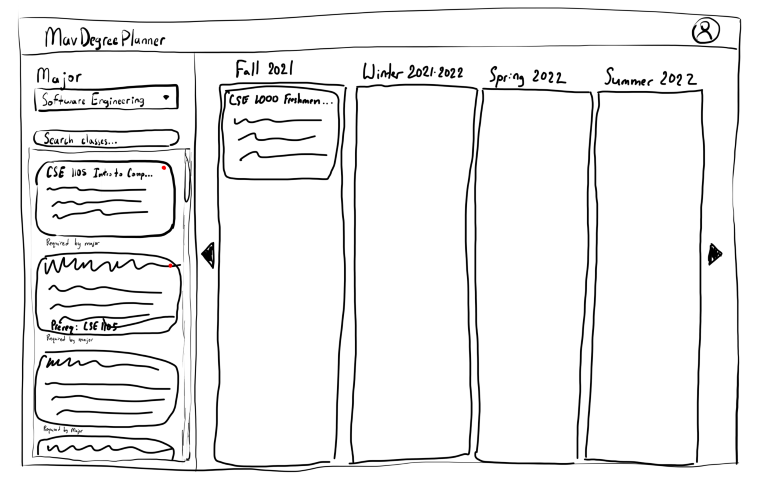
\includegraphics[width=0.60\textwidth]{images/MavDegreePlannerDiagram-Small}
\end{figure}
\vspace{0.5 in}
{\centering \huge \color{accentcolor} \sc \textbf{\teamname \\ \productname} \par}
\vspace{0.5 in}
{\centering \large \sc \textbf{\authors} \par}
\newpage


%\vspace{1 in}
%\centerline{January 13th, 2012}
%\newpage

%%% Revision History
\begin{versionhistory}
  	\vhEntry{0.1}{11.01.2021}{Group}{document creation}
  	\vhEntry{0.2}{11.05.2021}{Group}{document completion (Initial Release)}
\end{versionhistory}
\newpage

%%% Table of contents
\setcounter{tocdepth}{3}
\tableofcontents
\newpage

%%% List of figures and tables (optional)
\listoffigures
%\listoftables
\newpage

\section{Product Concept}
This section describes the purpose, use, and intended user audience for the Interactive Degree Planner. The basic concept of this web-based application is to assist UTA Computer Science and Engineering (CSE) students to create their degree planners that best fit their academic path. The website aims to provide the user-friendly interface taking advantage of drag-and-drop to simplify the degree planning process.

\subsection{Purpose and Use}
The Interactive Degree Planner website allows UTA students to register and log into the system. The users need to update their degree information before using the application. They are able to select the latest flow charts from the list of supported majors (i.e., Computer Science, Computer Engineering, and Software Engineering); this allows the website to offer the appropriate course catalog of the right major. Each course option in the provided list includes all important information, such as credit value, course title, course number, course description, and etc. Notably, these options are only available for the users as long as they fulfil the pre-/co-requisite and UTA is going to offer the class in the specific semester. The drag-and-drop pattern is implemented in the hope of facilitating the users' experience during the planning process. The users can freely modify their planners as long as no restriction is violated. Besides, the website  demonstrates essential information, including the total hours per semester and the estimated graduation date.

\subsection{Intended Audience}
The intended audience of this web-based application are current and/or future CSE students at the University of Texas at Arlington. Currently, the website are developed based on only three majors in the CSE department. However, all UTA students, who have different majors, are still able to use this website to build their possible-CSE planner as reference information.

\begin{figure}[h!]
	\centering
   	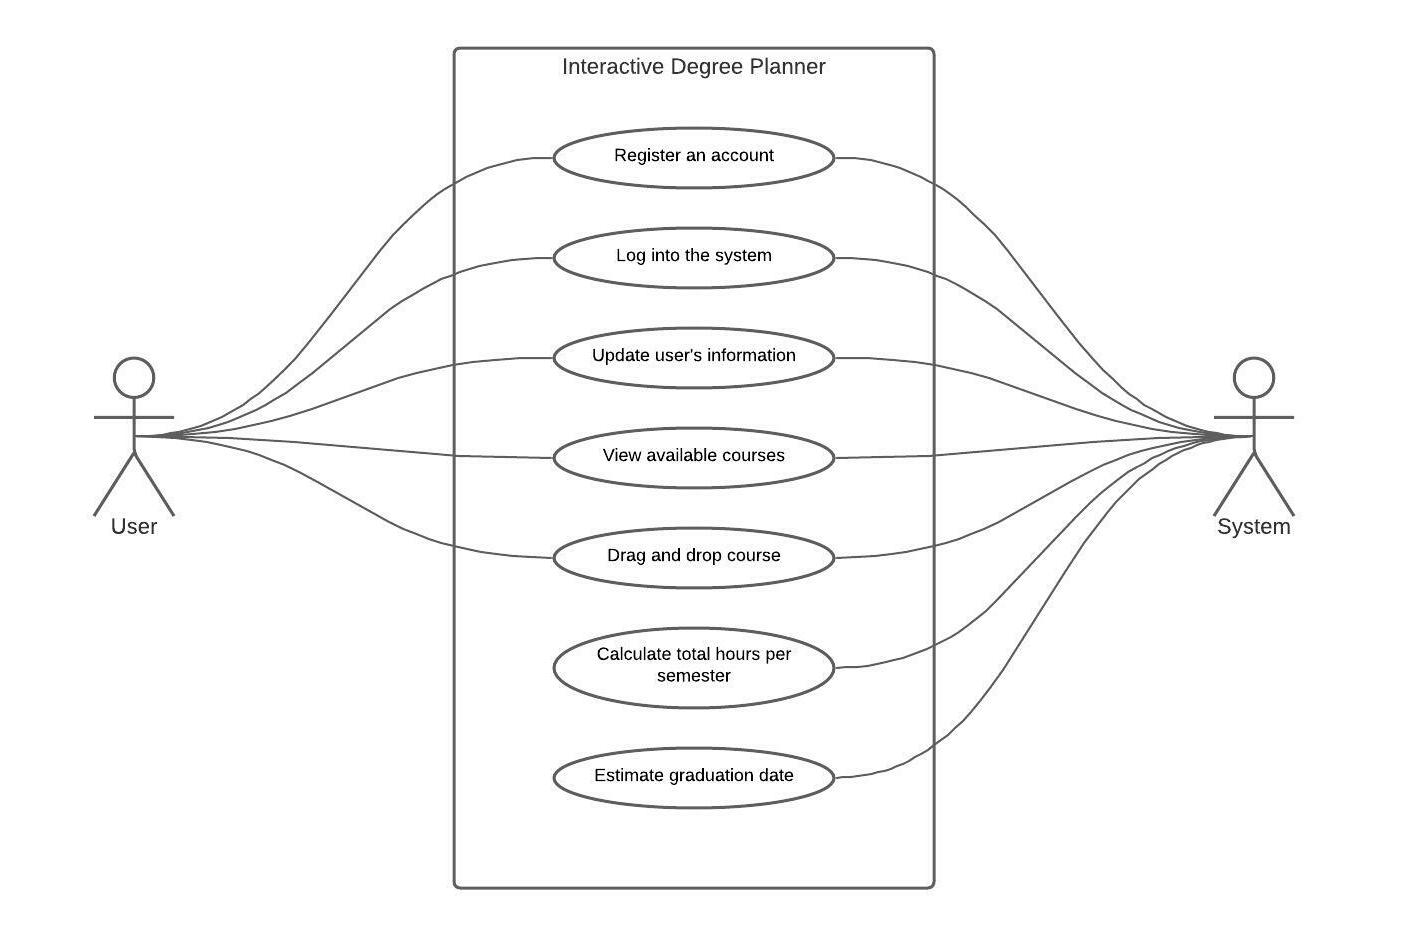
\includegraphics[width=0.60\textwidth]{images/uml}
    \caption{IDP conceptual drawing}
\end{figure}

\newpage
\section{Product Description}
% This section provides a description of your product and defines it's
% primary features and functions. The purpose is to give the document
% reader/reviewer enough information about the product to allow them
% to easily follow the specification of requirements found in the
% remainder of the document. Your header for this section should
% introduce the section with a brief statement such as: "This section
% provides the reader with an overview of X. The primary operational
% aspects of the product, from the perspective of end users, maintainers
% and administrators, are defined here. The key features and functions
% found in the product, as well as critical user interactions and user
% interfaces are described in detail." Using words, and pictures or
% graphics where possible, specify the following:

This section provides the reader with an overview of MavDegreePlanner.
The primary operational aspects of the product, from the perspective
of end users and maintainers are defined here. The key features and
functions found in the product, as well as critical user interactions
and user interfaces are described in detail.

\subsection{Features \& Functions}
% What the product does and does not do. Specify in words what it looks
% like, referring to a conceptual diagram/graphic (Figure X).  Define
% the principle parts/components of the product. Specify the elements
% in the diagram/graphic that are part(s) of this product as well as
% any associated external elements (e.g., the Internet, an external
% web server, a GPS satellite, etc.)

The screen is divided into two parts, the website banner, the side
panel and the main screen. The side panel has a button to select a
major, a search bar, and the list of classes. The main screen has
the list of semesters and which classes the student has selected
for each. The website banner has the website logo, title, and
a button to go to the accounts page.

Accounts page where users can sign in, sign out, and reset password.
Users can create an account so that they can access their degree plan
from any device.

In the side panel, show a list of classes which are draggable,
and visually show which classes are required by the degree plan.
Choosing a major will show which classes are required for the student
to take. The classes can also be searched using the search bar above the list.

On the main screen, show a row of semesters which classes can be dragged to.
The list of semesters can be horizonally scrolled to show more semesters, and
have buttons to scroll for the user.
Classes are chosen by dragging and droping classes to the semester box.
There will be an error shown to the user if they choosen a class
without having the co-reg or pre-req class.

\subsection{External Inputs \& Outputs}
Describe critical external data flows. What does your product
require/expect to receive from end users or external systems (inputs),
and what is expected to be created by your product for consumption by
end users or external systems (outputs)? In other words, specify here
all data/information to flow into and out of your systems. A table
works best here, with rows for each critical data element, and columns
for name, description and use.

\subsection{Product Interfaces}
Specify what all operational (visible) interfaces look like to your
end-user, administrator, maintainer, etc. Show sample/mocked-up screen shots,
graphics of buttons, panels, etc. Refer to the critical external inputs
and outputs described in the paragraph above.

\newpage
\section{Customer Requirements}
This section will speak about the customer requirements that we will be using the implement the web application.

\subsection{Registration}
\subsubsection{Description}
Initially, students must register the accounts in order to use the website. Required information includes emails, username, and password. Additional information may be asked, but not mandatory. After the registration succeeds, the students will be able to login to the website.
\subsubsection{Source}
Team Idea
\subsubsection{Constraints}
None
\subsubsection{Standards}
None
\subsubsection{Priority}
High

\subsection{Login}
\subsubsection{Description}
If the users are registered, he/she should be able to login in the system using the authenticated credential.
\subsubsection{Source}
Team Idea
\subsubsection{Constraints}
Students must be registered in the system.
\subsubsection{Standards}
None
\subsubsection{Priority}
High

\subsection{Drag and Drop}
\subsubsection{Description}
The web app will have a GUI which allows users to drag and drop classes into their degree plan. The drag and drop will allow a class to be clicked on and then dragged to the user's intended semester in which they will take the class, and finally dropped if that is the semester they intend to take that specific class.
\subsubsection{Source}
Team Idea
\subsubsection{Constraints}
A constraint for drag and drop is when the user drags a class and they let it go, if there is no valid place to drop that class into, then it should return to where it came from. It should drag and drop only to boxes that are intended to be filled. There should be a limit to where the drops can be made. For example, if the user drags a class and drops it in between two semesters, then it should not just drop there. Instead, it should choose the closer box or it should return back to where it came from. 
\subsubsection{Standards}
None
\subsubsection{Priority}
High

\subsection{Semesters}
\subsubsection{Description}
The web app will have sections of semesters. They will allow the users to add classes with the drag and drop feature allowing the user to plan their degree. The user can also take classes away from a semester and move it into another semester or back to the class list. 
\subsubsection{Source}
Team Idea
\subsubsection{Constraints}
Some constraints for this requirement are that there should only be a certain number of classes within a semester. Uta only permits 20 hours in a normal semester and 9 hours in a summer semester. The semester boxes will have to account for the amount of hours a student adds into it.  
\subsubsection{Standards}
None
\subsubsection{Priority}
High

\subsection{List of Classes}
\subsubsection{Description}
The app will have a list that contains all the classes that the user can select from. It will allow the user to select which classes they want to drag and drop into the desired semester that they choose. The list of classes will be ones that are offered at UTA. There will also be a search bar to make it easier for the user to search through the list and make it more easier to select a specific class that they have in mind. 
\subsubsection{Source}
Team Idea
\subsubsection{Constraints}
The list of classes will have constraints such as only listing classes that are offered at UTA. 
\subsubsection{Standards}
None
\subsubsection{Priority}
High

\subsection{Accounts}
\subsubsection{Description}
Users will all have their own degree plan. They can choose which classes they want in each semester. To make this happen, there needs to be accounts for the users to separate the data. This will allow the user to save their own unique data and give them access to create their degree plan in the order they choose. 
\subsubsection{Source}
Team Idea
\subsubsection{Constraints}
The account should be secured and data should not be leaked. Moreover, the users account credentials should be verified to make sure they are part of the UTA system. The user will need to be a UTA student or have valid UTA credentials, which will allow them to access the degree 
\subsubsection{Standards}
None
\subsubsection{Priority}
Medium

\subsection{Majors}
\subsubsection{Description}
The degree planner app must work off the major of the user. If the user has a different major then there should be a different list of classes for the user to drag and drop into semesters. There will be a selection box for the user to select their major and once the major is selected, the user will be able to drag and drop classes from the list that major has in order to complete that degree.  
\subsubsection{Source}
Team Idea
\subsubsection{Constraints}
Constraints for this requirement are that the user cannot add different classes from different majors. They are not allowed to mix and match. For example, the user can't select a business major and drag and drop classes into their semester if they already have another majors classes in their degree plan. The user is only allowed to select from the classes provided in that major alone.  
\subsubsection{Standards}
None
\subsubsection{Priority}
High

\subsection{Security}
\subsubsection{Description}
The website should provide secure service.
\subsubsection{Source}
Team Idea
\subsubsection{Constraints}
The information should be protected properly.
\subsubsection{Standards}
None
\subsubsection{Priority}
Medium


\newpage
\section{Packaging Requirements}
% Include a header paragraph here. Packaging requirements are
% those requirements that identify how the delivered product
% will be packaged for delivery to the end-user; or how it
% will "look" when finished and delivered. For example, you
% might specify that the software required for operation will
% be pre-loaded on the hard drive, delivered on CD/DVD, or
% available via download. Software might be customer installable,
% or not, etc. Hardware components could be all in a single
% package, provided as a "bag of parts" to be assembled/installed
% by the user, painted a certain color, logos affixed, etc. Care
% should be taken not to duplicate requirements found in other
% sections of this document.

This section details how the product will be delivered to the
end-users.

\subsection{Website}
\subsubsection{Description}
End-users can access the website from the given url.
\subsubsection{Source}
Team
\subsubsection{Constraints}
The server must be hosted and available to the internet.
\subsubsection{Standards}
No standards
\subsubsection{Priority}
High

\subsection{Source Code Download}
\subsubsection{Description}
The customer will be given a link to download a ZIP file with
the source code. Instructions will also be provided detailing
how to deploy it on a server or to view it locally.
\subsubsection{Source}
Team
\subsubsection{Constraints}
The ZIP file must be uploaded to the cloud so it can be shared
and downloaded.
\subsubsection{Standards}
The file is provided in ZIP format.
\subsubsection{Priority}
Low
\newpage
\section{Performance Requirements}
Include a header paragraph specific to your product here. Performance requirements address items such as: how fast specific critical operations must complete; how long it takes to start/stop activities; how long the battery must last; maximum time it must take to set up; etc.

\subsection{Requirement Name}
\subsubsection{Description}
Detailed requirement description...
\subsubsection{Source}
Source
\subsubsection{Constraints}
Detailed description of applicable constraints...
\subsubsection{Standards}
List of applicable standards
\subsubsection{Priority}
Priority
\newpage
\section{Safety Requirements}
This section will explain the safety requirements for the product which include things both software and hardware if applicable.\\
\subsection{Student Account Protection}
\subsubsection{Description}
As this is a software project that has no hardware units, this is the main safety requirement. This requirement of account safety is important as users will need to be sure that there information regarding what classes they've taken will remain in tact as well as stored safely.
\subsubsection{Source}
Team Idea
\subsubsection{Constraints}
Due to creating our own databases and not having access to the UTA Database and student information, we are limited to a basic account security without high level protection.
\subsubsection{Standards}
No Standards (Software Project)
\subsubsection{Priority}
High

\newpage
\section{Maintenance \& Support Requirements}
Include a header paragraph specific to your product here. Maintenance and support requirements address items specific to the ongoing maintenance and support of your product after delivery. Think of these requirements as if you were the ones who would be responsible for caring for customers/end user after the product is delivered in its final form and in use "in the field". What would you require to do this job? Specify items such as: where, how and who must be able to maintain the product to correct errors, hardware failures, etc.; required support/troubleshooting manuals/guides; availability/documentation of source code; related technical documentation that must be available for maintainers; specific/unique tools required for maintenance; specific software/environment required for maintenance; etc.

\subsection{Requirement Name}
\subsubsection{Description}
Detailed requirement description...
\subsubsection{Source}
Source
\subsubsection{Constraints}
Detailed description of applicable constraints...
\subsubsection{Standards}
List of applicable standards
\subsubsection{Priority}
Priority
\newpage
\section{Other Requirements}
Include a header paragraph specific to your product here. In this section specify anything else that is required for the product to be deemed complete. Include requirements related to customer setup and configuration if not specified in a previous requirement. Add any known requirements related to product architecture/design, such as modularity, extensibility (for future enhancements), or adaptation for a specific programming language. Consider requirements such as portability of your source code to various platforms (Windows, Linux, Unix Mac OS, etc.).

\subsection{Requirement Name}
\subsubsection{Description}
Detailed requirement description...
\subsubsection{Source}
Source
\subsubsection{Constraints}
Detailed description of applicable constraints...
\subsubsection{Standards}
List of applicable standards
\subsubsection{Priority}
Priority
\newpage
\section{Future Items}
Currently, the Interactive Degree Planner is solely a web-based application targeting students from Computer Science and Engineering department at the University of Texas at Arlington. Therefore, we are expecting to expand the service in the future, such as providing detail degree planner for majors other than CSE and making an mobile application of this.

\subsection{Non-CSE Degree Planner}
\subsubsection{Description}
We hope to make the application available to all departments at UTA, so that all students are able to acknowledge their academic paths in the easier, faster, and more efficient way.
\subsubsection{Source}
Team Idea
\subsubsection{Constraints}
We might need the comprehensive instruction from the faculties of different departments to build the most appropriate degree planner.
\subsubsection{Standards}
N/A
\subsubsection{Priority}
Medium

\subsection{Mobile Application}
\subsubsection{Description}
Due to constraints of time, skills, and feasibility analysis, we decide not to focus on the mobile application for now. However, this is a potential development in the future, which allows users to access to the service easier.
\subsubsection{Source}
Team Idea
\subsubsection{Constraints}
Specific skills and tools about mobile application must be acknowledged (i.e., Android Studio for Android application, and/or Swift for iOS).
\subsubsection{Standards}
N/A
\subsubsection{Priority}
Medium
\newpage

%%% References
\bibliographystyle{plain}
\bibliographystyle{reference/IEEEtran_custom}
\nocite{*} % https://tex.stackexchange.com/questions/205176/empty-thebibliography-environment
\bibliography{reference/refs}

\end{document}